\documentclass{article}
\usepackage{tikz, comment}
\usepackage{pifont}
\usepackage{fontspec, pgfplots}
\usetikzlibrary{arrows, decorations.markings, decorations.pathreplacing}
\begin{comment}
:Title: Not defined yet
:Tags: absolute value rules;deleted neighborhood;inverse of a matrix, matrix inverse , multiplicative inverse of a matrix ;neighborhood;equation of a line
:Prob: 0.5418;0.5226;0.5187;0.5179;0.5151
:Author: Prof.Hu Ji-shan, HKUST
:Slug: No name yet

Description Here.........
\end{comment}
\begin{document}\centering 

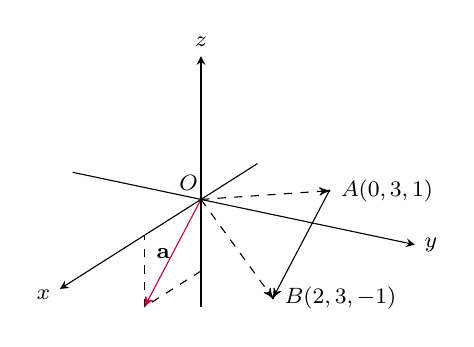
\begin{tikzpicture}[font=\footnotesize]
\pgfplotsset{compat=1.8}
\begin{axis}
[axis lines = center, view={120}{30}, ticks=none, 
axis on top, xlabel = {$x$}, ylabel ={$y$}, zlabel ={$z$}, domain =0:1, y domain =0:1,
xmin =-2.0,
xmax =5.0,
ymin =-3.0,
ymax =5,
zmin =-3.0, 
zmax =4.0,
samples =10, samples y =40, z buffer =sort,
every axis x label/.style={
    at={(ticklabel* cs:1)},
    anchor= east, yshift =-2
},
every axis y label/.style={
    at={(ticklabel* cs:1)},
    anchor= west,
},
every axis z label/.style={
    at={(ticklabel* cs:1)},
    anchor= south
}]

\node[label={0:{$A(0,3,1)$}},circle,fill,inner sep=0pt] at (axis cs:0,3,1) {};
\node[label={0:{$B(2,3,-1)$}},circle,fill,inner sep=0pt] at (axis cs:2,3,-1) {};

\node[xshift=6, label={180:{${\bf a}$}}] at (axis cs:1,0,-1) {};

\node[xshift=3, yshift=-4, label={100:{$O$}}] at (axis cs:0,0,0) {};

\addplot3[dashed, ->, >=stealth'] coordinates
        {(0,0,0) (0,3,1)};

\addplot3[dashed, ->, >=stealth'] coordinates
        {(0,0,0) (2,3,-1)};

\addplot3[->, >=stealth'] coordinates
        {(0,3,1) (2,3,-1)};

\addplot3[purple, ->, >=stealth'] coordinates
        {(0,0,0) (2,0,-2)};

\addplot3[dashed] coordinates
        {(2,0,-2) (0,0,-2)};
\addplot3[dashed] coordinates
        {(2,0,-2) (2,0,-2)};
\addplot3[dashed] coordinates
        {(2,0,-2) (2,0,0)};

\end{axis}

\end{tikzpicture}
\end{document}